\section{Results}

\begin{figure*}[htbp]
\centerline{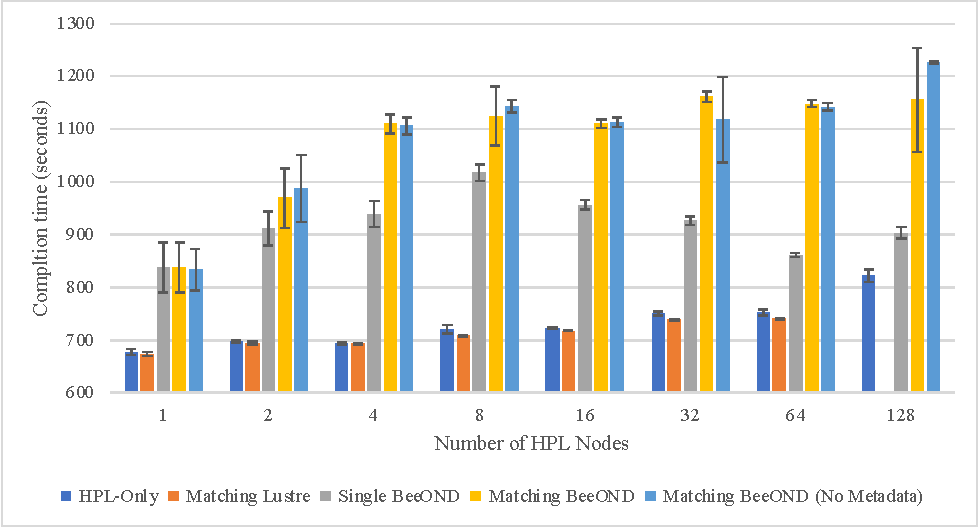
\includegraphics{multinode-hpl-runtime-impact}}
\caption{Execution times of HPL with and without IOR processes co-located within the partition. Error bars indicate 95\% confidence interval.}
\label{fig:multinode}
\end{figure*}

This set of experiment included a small set of anomalies that we note here for completeness, but do not affect our analysis. All runs were completed between 7 and 10 times, with few exceptions. First, since we anticipated the ``Matching Lustre'' cases to be less variable, we only ran those experiments only three times each. Second, we were unable to get the largest Lustre run category (128-node HPL + 128-node IOR) completed before the deadline, as the system is a busy production platform. We will include this last data point before final publication. In the case of the 128-node HPL+BeeOND executions, we occasionally experienced runtimes slightly longer than the 20-minute IOR limit. We believe this did not significantly impact measurements, as the average runtime was less than 5\% longer than 20 minutes.

\begin{figure}[htbp]
\centerline{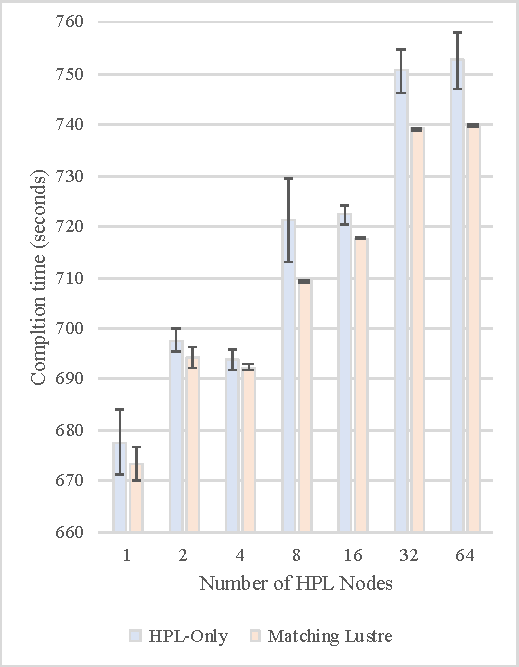
\includegraphics{multinode-95ci-lustre-beeond}}
\caption{A detailed view of HPL execution variance between HPL-only tasks (with BeeOND processes running) and HPL running alongside IOR targetting Lustre (without BeeOND processes running).}
\label{multinode-variance}
\end{figure}

{\bf Overall trends.} Based on our full results, shown in Figure~\ref{fig:multinode}, it is clear that introducing a storage workload on BeeOND daemons running alongside HPL cause statistically significant impact to HPL runtime. Introducing a single IOR process affected jobs of all sizes, causing the HPL-only job to increase its runtime by 7-13\% for 128 processes. Further increasing the I/O load with matching processes caused even greater execution times, with the 128-node Matching BeeOND (No Metadata) case experiencing 47-52\% extended runtime.

{\bf Metadata server effects.} In the ``Beeond Matching, Skip Metadata'' experiments, we were sure to keep the multi-node HPL from running on the node that hosted the metadata server. This was in contrast to the ``BeeOND Matching,'' where the multi-node HPL would overlap with the metadata server. The intention was to separate additional metadata tasks caused by our IOR workload to be from measurement, showing whether object storage processes caused less runtime impact generally. Our experiments did not definitively demonstrate a difference runtime. Determining the extent of any impact will require further experimentation focusing on metadata workloads, as well as how different types of workloads may be balanced by BeeOND.

{\bf Overhead of idle BeeOND daemons.} Figure~\ref{multinode-variance} shows a detailed view of a particularly interesting phenomenon. When running HPL-only configurations, we used the same job scripts that were used for BeeOND-enabled IOR tests. Therefore, the same Slurm constraint that caused BeeOND startup were included, so those processes were running on those nodes. However, for the Lustre-specific runs, we did not specify the BeeOND constraint, so did not load any BeeOND daemons. Despite a total absence of storage operations during the HPL-only jobs, the HPL-only jobs were slower than the Lustre+IOR jobs by a statistically significant margin. For the 64-node HPL cases, this impact was likely between 0.9 and 2.5\%. This impact grows with the size of the job, indicating that large scale runs could see even larger slowdowns. This is congruent with findings from previous work that showed daemon processes on Linux clusters could consume enough cycles to impact larger scale tasks~\cite{daemon-interference}. This was a surprising finding, and we intend to pursue this line of investigation further. While the confounding factor of the Lustre IOR prevents us from definitively asserting that idle BeeOND daemons caused an overhead, a simple variation of this experiment will definitively show whether this link exists. Such an experiment will be run and reported for an accepted version of this paper.
